\begin{figure}[h]
    \centering
    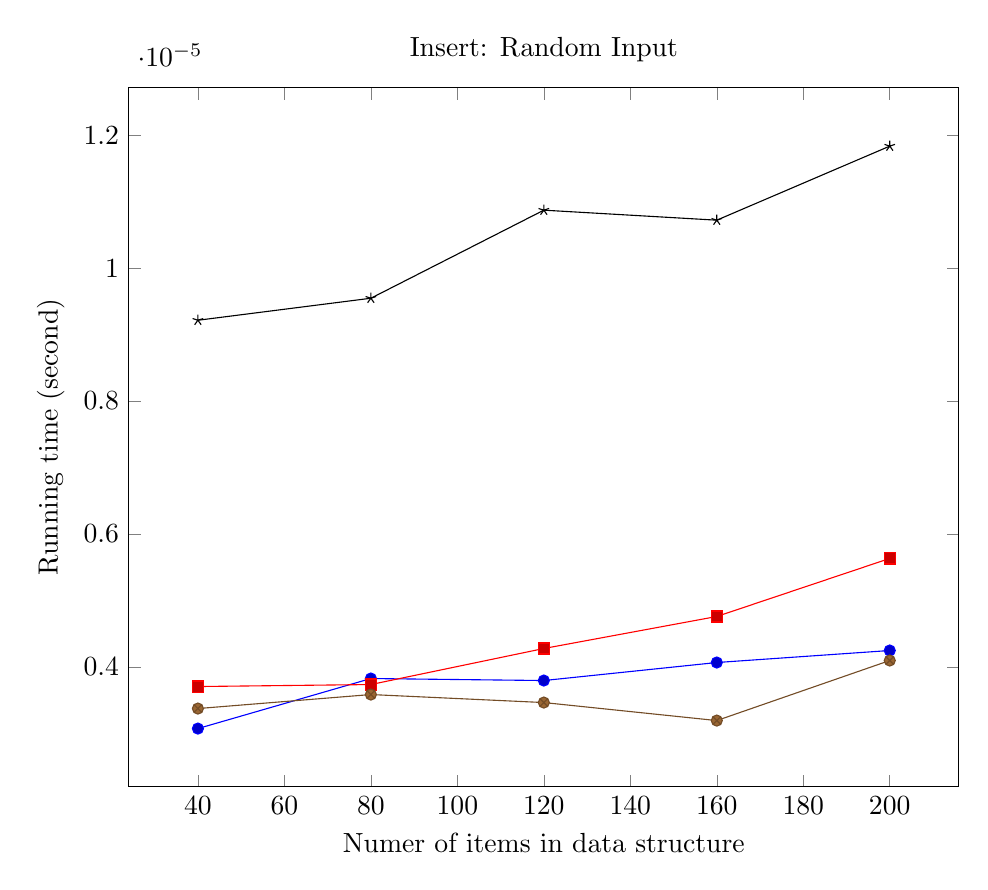
\begin{tikzpicture}
        \begin{axis}[
            xlabel={Numer of items in data structure},
            ylabel={Running time (second)},
            title={Insert: Random Input},
            width=\textwidth
        ]
		\addplot coordinates {
			(200, 4.2465722481985905e-06)
			(160, 4.065867046147567e-06)
			(120, 3.7948092430710545e-06)
			(80, 3.824926776746246e-06)
			(40, 3.071988434867048e-06)
		};
		\addplot coordinates {
			(200, 5.631978797256305e-06)
			(160, 4.758570320676468e-06)
			(120, 4.276689781873739e-06)
			(80, 3.7345741757208e-06)
			(40, 3.7044566420455644e-06)
		};
		\addplot coordinates {
			(200, 4.095984579822673e-06)
			(160, 3.192458569567687e-06)
			(120, 3.4635163726442e-06)
			(80, 3.5839865073449688e-06)
			(40, 3.3731637716187535e-06)
		};
		\addplot coordinates {
			(200, 1.1836190734340787e-05)
			(160, 1.0721841988359585e-05)
			(120, 1.0872429656735329e-05)
			(80, 9.547258175028258e-06)
			(40, 9.2159653046011e-06)
		};
        \legend{}
        \end{axis}
    \end{tikzpicture}
    \caption{Average of 0 operations, benchmarked every 0, starting at 0.}
\end{figure}